% Created by tikzDevice version 0.12.6 on 2025-02-07 13:03:39
% !TEX encoding = UTF-8 Unicode
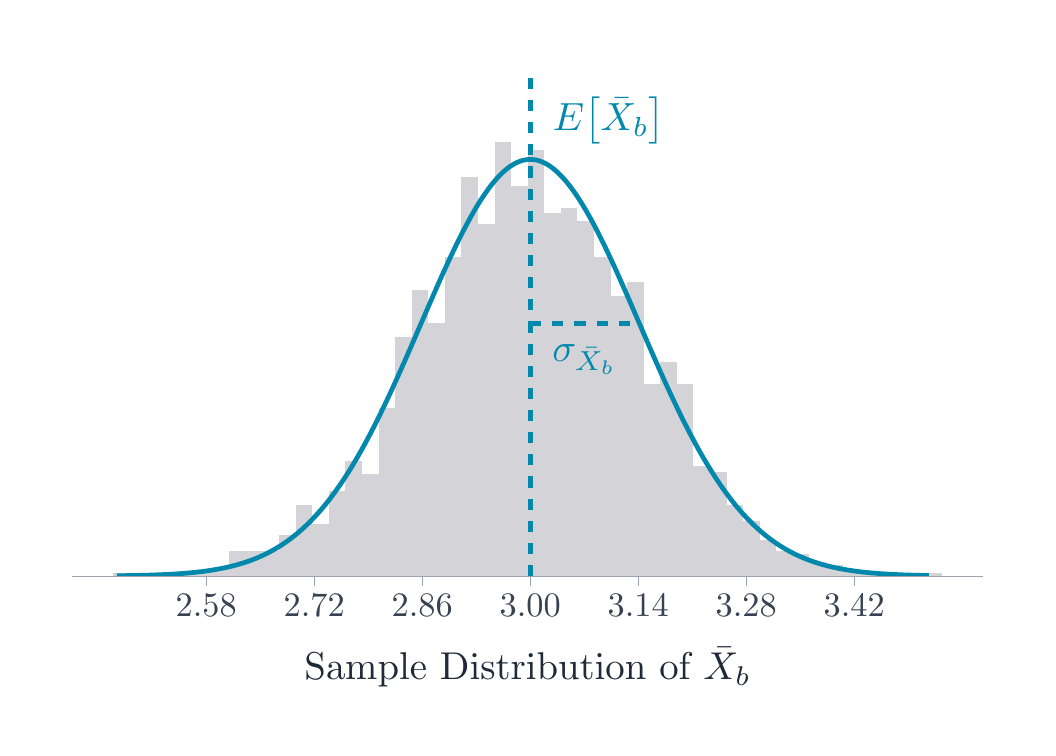
\begin{tikzpicture}[x=1pt,y=1pt]
\definecolor{fillColor}{RGB}{255,255,255}
\path[use as bounding box,fill=fillColor] (0,0) rectangle (361.35,252.94);
\begin{scope}
\path[clip] (  0.00,  0.00) rectangle (361.35,252.94);
\definecolor{drawColor}{RGB}{255,255,255}

\path[draw=drawColor,line width= 0.7pt,line join=round,line cap=round,fill=fillColor] (  0.00,  0.00) rectangle (361.35,252.94);
\end{scope}
\begin{scope}
\path[clip] ( 16.00, 54.78) rectangle (345.35,236.94);
\definecolor{drawColor}{RGB}{255,255,255}
\definecolor{fillColor}{RGB}{255,255,255}

\path[draw=drawColor,line width= 0.7pt,line join=round,line cap=round,fill=fillColor] ( 16.00, 54.78) rectangle (345.35,236.94);
\definecolor{fillColor}{RGB}{212,212,216}

\path[fill=fillColor] ( 30.97, 54.78) rectangle ( 36.96, 55.78);

\path[fill=fillColor] ( 36.96, 54.78) rectangle ( 42.95, 55.78);

\path[fill=fillColor] ( 42.95, 54.78) rectangle ( 48.94, 54.78);

\path[fill=fillColor] ( 48.94, 54.78) rectangle ( 54.92, 55.78);

\path[fill=fillColor] ( 54.92, 54.78) rectangle ( 60.91, 55.78);

\path[fill=fillColor] ( 60.91, 54.78) rectangle ( 66.90, 56.77);

\path[fill=fillColor] ( 66.90, 54.78) rectangle ( 72.89, 57.77);

\path[fill=fillColor] ( 72.89, 54.78) rectangle ( 78.88, 63.73);

\path[fill=fillColor] ( 78.88, 54.78) rectangle ( 84.86, 63.73);

\path[fill=fillColor] ( 84.86, 54.78) rectangle ( 90.85, 63.73);

\path[fill=fillColor] ( 90.85, 54.78) rectangle ( 96.84, 69.69);

\path[fill=fillColor] ( 96.84, 54.78) rectangle (102.83, 80.62);

\path[fill=fillColor] (102.83, 54.78) rectangle (108.82, 73.66);

\path[fill=fillColor] (108.82, 54.78) rectangle (114.81, 85.59);

\path[fill=fillColor] (114.81, 54.78) rectangle (120.79, 96.52);

\path[fill=fillColor] (120.79, 54.78) rectangle (126.78, 91.55);

\path[fill=fillColor] (126.78, 54.78) rectangle (132.77,115.40);

\path[fill=fillColor] (132.77, 54.78) rectangle (138.76,141.24);

\path[fill=fillColor] (138.76, 54.78) rectangle (144.75,158.13);

\path[fill=fillColor] (144.75, 54.78) rectangle (150.73,146.21);

\path[fill=fillColor] (150.73, 54.78) rectangle (156.72,170.06);

\path[fill=fillColor] (156.72, 54.78) rectangle (162.71,198.87);

\path[fill=fillColor] (162.71, 54.78) rectangle (168.70,181.98);

\path[fill=fillColor] (168.70, 54.78) rectangle (174.69,211.79);

\path[fill=fillColor] (174.69, 54.78) rectangle (180.68,195.89);

\path[fill=fillColor] (180.68, 54.78) rectangle (186.66,208.81);

\path[fill=fillColor] (186.66, 54.78) rectangle (192.65,185.95);

\path[fill=fillColor] (192.65, 54.78) rectangle (198.64,187.94);

\path[fill=fillColor] (198.64, 54.78) rectangle (204.63,182.97);

\path[fill=fillColor] (204.63, 54.78) rectangle (210.62,170.06);

\path[fill=fillColor] (210.62, 54.78) rectangle (216.60,156.14);

\path[fill=fillColor] (216.60, 54.78) rectangle (222.59,161.11);

\path[fill=fillColor] (222.59, 54.78) rectangle (228.58,124.34);

\path[fill=fillColor] (228.58, 54.78) rectangle (234.57,132.29);

\path[fill=fillColor] (234.57, 54.78) rectangle (240.56,124.34);

\path[fill=fillColor] (240.56, 54.78) rectangle (246.54, 94.53);

\path[fill=fillColor] (246.54, 54.78) rectangle (252.53, 92.55);

\path[fill=fillColor] (252.53, 54.78) rectangle (258.52, 80.62);

\path[fill=fillColor] (258.52, 54.78) rectangle (264.51, 74.66);

\path[fill=fillColor] (264.51, 54.78) rectangle (270.50, 67.70);

\path[fill=fillColor] (270.50, 54.78) rectangle (276.49, 63.73);

\path[fill=fillColor] (276.49, 54.78) rectangle (282.47, 62.73);

\path[fill=fillColor] (282.47, 54.78) rectangle (288.46, 59.75);

\path[fill=fillColor] (288.46, 54.78) rectangle (294.45, 58.76);

\path[fill=fillColor] (294.45, 54.78) rectangle (300.44, 56.77);

\path[fill=fillColor] (300.44, 54.78) rectangle (306.43, 55.78);

\path[fill=fillColor] (306.43, 54.78) rectangle (312.42, 54.78);

\path[fill=fillColor] (312.41, 54.78) rectangle (318.40, 55.78);

\path[fill=fillColor] (318.40, 54.78) rectangle (324.39, 54.78);

\path[fill=fillColor] (324.39, 54.78) rectangle (330.38, 55.78);
\definecolor{drawColor}{RGB}{1,136,172}

\path[draw=drawColor,line width= 1.7pt,line join=round] ( 32.21, 54.90) --
	( 33.19, 54.91) --
	( 34.18, 54.92) --
	( 35.16, 54.94) --
	( 36.14, 54.95) --
	( 37.12, 54.97) --
	( 38.10, 54.98) --
	( 39.08, 55.00) --
	( 40.06, 55.02) --
	( 41.05, 55.05) --
	( 42.03, 55.07) --
	( 43.01, 55.10) --
	( 43.99, 55.12) --
	( 44.97, 55.16) --
	( 45.95, 55.19) --
	( 46.93, 55.23) --
	( 47.92, 55.26) --
	( 48.90, 55.31) --
	( 49.88, 55.35) --
	( 50.86, 55.40) --
	( 51.84, 55.45) --
	( 52.82, 55.51) --
	( 53.80, 55.57) --
	( 54.78, 55.64) --
	( 55.77, 55.71) --
	( 56.75, 55.78) --
	( 57.73, 55.87) --
	( 58.71, 55.95) --
	( 59.69, 56.05) --
	( 60.67, 56.15) --
	( 61.65, 56.26) --
	( 62.64, 56.37) --
	( 63.62, 56.49) --
	( 64.60, 56.63) --
	( 65.58, 56.77) --
	( 66.56, 56.92) --
	( 67.54, 57.08) --
	( 68.52, 57.25) --
	( 69.50, 57.43) --
	( 70.49, 57.62) --
	( 71.47, 57.83) --
	( 72.45, 58.05) --
	( 73.43, 58.28) --
	( 74.41, 58.52) --
	( 75.39, 58.78) --
	( 76.37, 59.06) --
	( 77.36, 59.35) --
	( 78.34, 59.66) --
	( 79.32, 59.99) --
	( 80.30, 60.33) --
	( 81.28, 60.70) --
	( 82.26, 61.08) --
	( 83.24, 61.49) --
	( 84.22, 61.92) --
	( 85.21, 62.36) --
	( 86.19, 62.84) --
	( 87.17, 63.34) --
	( 88.15, 63.86) --
	( 89.13, 64.41) --
	( 90.11, 64.98) --
	( 91.09, 65.58) --
	( 92.08, 66.22) --
	( 93.06, 66.88) --
	( 94.04, 67.57) --
	( 95.02, 68.29) --
	( 96.00, 69.05) --
	( 96.98, 69.83) --
	( 97.96, 70.65) --
	( 98.94, 71.51) --
	( 99.93, 72.40) --
	(100.91, 73.33) --
	(101.89, 74.29) --
	(102.87, 75.29) --
	(103.85, 76.33) --
	(104.83, 77.41) --
	(105.81, 78.52) --
	(106.80, 79.68) --
	(107.78, 80.87) --
	(108.76, 82.11) --
	(109.74, 83.39) --
	(110.72, 84.70) --
	(111.70, 86.06) --
	(112.68, 87.46) --
	(113.66, 88.91) --
	(114.65, 90.39) --
	(115.63, 91.92) --
	(116.61, 93.49) --
	(117.59, 95.09) --
	(118.57, 96.74) --
	(119.55, 98.43) --
	(120.53,100.16) --
	(121.52,101.93) --
	(122.50,103.74) --
	(123.48,105.58) --
	(124.46,107.47) --
	(125.44,109.38) --
	(126.42,111.34) --
	(127.40,113.32) --
	(128.39,115.34) --
	(129.37,117.39) --
	(130.35,119.47) --
	(131.33,121.58) --
	(132.31,123.71) --
	(133.29,125.87) --
	(134.27,128.05) --
	(135.25,130.24) --
	(136.24,132.46) --
	(137.22,134.69) --
	(138.20,136.94) --
	(139.18,139.19) --
	(140.16,141.46) --
	(141.14,143.73) --
	(142.12,146.00) --
	(143.11,148.27) --
	(144.09,150.54) --
	(145.07,152.81) --
	(146.05,155.06) --
	(147.03,157.31) --
	(148.01,159.53) --
	(148.99,161.75) --
	(149.97,163.94) --
	(150.96,166.10) --
	(151.94,168.24) --
	(152.92,170.35) --
	(153.90,172.42) --
	(154.88,174.46) --
	(155.86,176.46) --
	(156.84,178.41) --
	(157.83,180.32) --
	(158.81,182.18) --
	(159.79,183.99) --
	(160.77,185.74) --
	(161.75,187.43) --
	(162.73,189.06) --
	(163.71,190.63) --
	(164.69,192.12) --
	(165.68,193.55) --
	(166.66,194.91) --
	(167.64,196.20) --
	(168.62,197.40) --
	(169.60,198.53) --
	(170.58,199.58) --
	(171.56,200.54) --
	(172.55,201.42) --
	(173.53,202.22) --
	(174.51,202.92) --
	(175.49,203.54) --
	(176.47,204.07) --
	(177.45,204.50) --
	(178.43,204.85) --
	(179.41,205.10) --
	(180.40,205.26) --
	(181.38,205.33) --
	(182.36,205.30) --
	(183.34,205.18) --
	(184.32,204.97) --
	(185.30,204.66) --
	(186.28,204.27) --
	(187.27,203.78) --
	(188.25,203.20) --
	(189.23,202.53) --
	(190.21,201.77) --
	(191.19,200.93) --
	(192.17,200.00) --
	(193.15,198.99) --
	(194.13,197.89) --
	(195.12,196.72) --
	(196.10,195.47) --
	(197.08,194.14) --
	(198.06,192.74) --
	(199.04,191.27) --
	(200.02,189.74) --
	(201.00,188.13) --
	(201.99,186.47) --
	(202.97,184.74) --
	(203.95,182.96) --
	(204.93,181.12) --
	(205.91,179.24) --
	(206.89,177.30) --
	(207.87,175.32) --
	(208.85,173.30) --
	(209.84,171.24) --
	(210.82,169.15) --
	(211.80,167.02) --
	(212.78,164.87) --
	(213.76,162.68) --
	(214.74,160.48) --
	(215.72,158.26) --
	(216.71,156.02) --
	(217.69,153.77) --
	(218.67,151.51) --
	(219.65,149.24) --
	(220.63,146.97) --
	(221.61,144.70) --
	(222.59,142.43) --
	(223.58,140.16) --
	(224.56,137.90) --
	(225.54,135.65) --
	(226.52,133.41) --
	(227.50,131.19) --
	(228.48,128.98) --
	(229.46,126.80) --
	(230.44,124.63) --
	(231.43,122.49) --
	(232.41,120.37) --
	(233.39,118.28) --
	(234.37,116.22) --
	(235.35,114.18) --
	(236.33,112.18) --
	(237.31,110.22) --
	(238.30,108.28) --
	(239.28,106.38) --
	(240.26,104.52) --
	(241.24,102.70) --
	(242.22,100.91) --
	(243.20, 99.17) --
	(244.18, 97.46) --
	(245.16, 95.79) --
	(246.15, 94.17) --
	(247.13, 92.58) --
	(248.11, 91.04) --
	(249.09, 89.54) --
	(250.07, 88.08) --
	(251.05, 86.66) --
	(252.03, 85.28) --
	(253.02, 83.94) --
	(254.00, 82.65) --
	(254.98, 81.40) --
	(255.96, 80.18) --
	(256.94, 79.01) --
	(257.92, 77.88) --
	(258.90, 76.78) --
	(259.88, 75.73) --
	(260.87, 74.71) --
	(261.85, 73.73) --
	(262.83, 72.79) --
	(263.81, 71.89) --
	(264.79, 71.02) --
	(265.77, 70.18) --
	(266.75, 69.38) --
	(267.74, 68.61) --
	(268.72, 67.87) --
	(269.70, 67.17) --
	(270.68, 66.50) --
	(271.66, 65.85) --
	(272.64, 65.24) --
	(273.62, 64.65) --
	(274.60, 64.09) --
	(275.59, 63.56) --
	(276.57, 63.05) --
	(277.55, 62.56) --
	(278.53, 62.10) --
	(279.51, 61.67) --
	(280.49, 61.25) --
	(281.47, 60.86) --
	(282.46, 60.49) --
	(283.44, 60.13) --
	(284.42, 59.80) --
	(285.40, 59.48) --
	(286.38, 59.18) --
	(287.36, 58.90) --
	(288.34, 58.63) --
	(289.32, 58.38) --
	(290.31, 58.14) --
	(291.29, 57.92) --
	(292.27, 57.71) --
	(293.25, 57.51) --
	(294.23, 57.32) --
	(295.21, 57.15) --
	(296.19, 56.98) --
	(297.18, 56.83) --
	(298.16, 56.69) --
	(299.14, 56.55) --
	(300.12, 56.42) --
	(301.10, 56.30) --
	(302.08, 56.19) --
	(303.06, 56.09) --
	(304.05, 55.99) --
	(305.03, 55.90) --
	(306.01, 55.82) --
	(306.99, 55.74) --
	(307.97, 55.67) --
	(308.95, 55.60) --
	(309.93, 55.54) --
	(310.91, 55.48) --
	(311.90, 55.42) --
	(312.88, 55.37) --
	(313.86, 55.33) --
	(314.84, 55.28) --
	(315.82, 55.24) --
	(316.80, 55.20) --
	(317.78, 55.17) --
	(318.77, 55.14) --
	(319.75, 55.11) --
	(320.73, 55.08) --
	(321.71, 55.06) --
	(322.69, 55.03) --
	(323.67, 55.01) --
	(324.65, 54.99) --
	(325.63, 54.97);

\path[draw=drawColor,line width= 1.7pt,dash pattern=on 4pt off 4pt ,line join=round] (181.59, 54.78) -- (181.59,236.94);

\path[] (188.10,211.43) --
	(230.38,211.43) --
	(230.27,211.44) --
	(230.69,211.45) --
	(231.09,211.54) --
	(231.48,211.68) --
	(231.84,211.89) --
	(232.16,212.15) --
	(232.43,212.46) --
	(232.65,212.81) --
	(232.81,213.19) --
	(232.91,213.59) --
	(232.95,214.00) --
	(232.95,214.00) --
	(232.95,226.77) --
	(232.95,226.77) --
	(232.91,227.18) --
	(232.81,227.58) --
	(232.65,227.96) --
	(232.43,228.31) --
	(232.16,228.62) --
	(231.84,228.88) --
	(231.48,229.09) --
	(231.09,229.23) --
	(230.69,229.32) --
	(230.38,229.34) --
	(188.10,229.34) --
	(188.41,229.32) --
	(188.00,229.33) --
	(187.59,229.28) --
	(187.19,229.17) --
	(186.81,228.99) --
	(186.47,228.76) --
	(186.18,228.47) --
	(185.93,228.14) --
	(185.73,227.77) --
	(185.60,227.38) --
	(185.54,226.97) --
	(185.53,226.77) --
	(185.53,214.00) --
	(185.54,214.21) --
	(185.54,213.80) --
	(185.60,213.39) --
	(185.73,213.00) --
	(185.93,212.63) --
	(186.18,212.30) --
	(186.47,212.01) --
	(186.81,211.78) --
	(187.19,211.60) --
	(187.59,211.49) --
	(188.00,211.44) --
	cycle;
\end{scope}
\begin{scope}
\path[clip] ( 16.00, 54.78) rectangle (345.35,236.94);
\definecolor{drawColor}{RGB}{1,136,172}

\node[text=drawColor,anchor=base west,inner sep=0pt, outer sep=0pt, scale=  1.42] at (189.81,215.72) {$\mathbb{E}\big[\bar{X}_b\big]$};
\end{scope}
\begin{scope}
\path[clip] ( 16.00, 54.78) rectangle (345.35,236.94);
\definecolor{drawColor}{RGB}{1,136,172}

\path[draw=drawColor,line width= 1.7pt,dash pattern=on 4pt off 4pt ,line join=round] (181.59,146.10) -- (221.01,146.10);

\path[] (187.89,128.19) --
	(214.71,128.19) --
	(214.60,128.19) --
	(215.02,128.21) --
	(215.42,128.29) --
	(215.81,128.44) --
	(216.17,128.65) --
	(216.49,128.91) --
	(216.76,129.22) --
	(216.98,129.57) --
	(217.15,129.95) --
	(217.24,130.35) --
	(217.28,130.76) --
	(217.28,130.76) --
	(217.28,143.52) --
	(217.28,143.52) --
	(217.24,143.94) --
	(217.15,144.34) --
	(216.98,144.72) --
	(216.76,145.07) --
	(216.49,145.38) --
	(216.17,145.64) --
	(215.81,145.85) --
	(215.42,145.99) --
	(215.02,146.08) --
	(214.71,146.10) --
	(187.89,146.10) --
	(188.20,146.08) --
	(187.78,146.09) --
	(187.37,146.04) --
	(186.98,145.93) --
	(186.60,145.75) --
	(186.26,145.52) --
	(185.96,145.23) --
	(185.72,144.90) --
	(185.52,144.53) --
	(185.39,144.14) --
	(185.33,143.73) --
	(185.32,143.52) --
	(185.32,130.76) --
	(185.33,130.97) --
	(185.33,130.56) --
	(185.39,130.15) --
	(185.52,129.76) --
	(185.72,129.39) --
	(185.96,129.06) --
	(186.26,128.77) --
	(186.60,128.54) --
	(186.98,128.36) --
	(187.37,128.24) --
	(187.78,128.19) --
	cycle;
\end{scope}
\begin{scope}
\path[clip] ( 16.00, 54.78) rectangle (345.35,236.94);
\definecolor{drawColor}{RGB}{1,136,172}

\node[text=drawColor,anchor=base,inner sep=0pt, outer sep=0pt, scale=  1.42] at (201.30,132.48) {$\sigma_{\bar{X}_b}$};
\end{scope}
\begin{scope}
\path[clip] (  0.00,  0.00) rectangle (361.35,252.94);
\definecolor{drawColor}{RGB}{156,163,175}

\path[draw=drawColor,line width= 0.3pt,line join=round] ( 16.00, 54.78) --
	(345.35, 54.78);
\end{scope}
\begin{scope}
\path[clip] (  0.00,  0.00) rectangle (361.35,252.94);
\definecolor{drawColor}{RGB}{156,163,175}

\path[draw=drawColor,line width= 0.3pt,line join=round] ( 64.51, 51.28) --
	( 64.51, 54.78);

\path[draw=drawColor,line width= 0.3pt,line join=round] (103.54, 51.28) --
	(103.54, 54.78);

\path[draw=drawColor,line width= 0.3pt,line join=round] (142.56, 51.28) --
	(142.56, 54.78);

\path[draw=drawColor,line width= 0.3pt,line join=round] (181.59, 51.28) --
	(181.59, 54.78);

\path[draw=drawColor,line width= 0.3pt,line join=round] (220.61, 51.28) --
	(220.61, 54.78);

\path[draw=drawColor,line width= 0.3pt,line join=round] (259.64, 51.28) --
	(259.64, 54.78);

\path[draw=drawColor,line width= 0.3pt,line join=round] (298.66, 51.28) --
	(298.66, 54.78);
\end{scope}
\begin{scope}
\path[clip] (  0.00,  0.00) rectangle (361.35,252.94);
\definecolor{drawColor}{RGB}{55,65,81}

\node[text=drawColor,anchor=base,inner sep=0pt, outer sep=0pt, scale=  1.24] at ( 64.51, 40.32) {2.58};

\node[text=drawColor,anchor=base,inner sep=0pt, outer sep=0pt, scale=  1.24] at (103.54, 40.32) {2.72};

\node[text=drawColor,anchor=base,inner sep=0pt, outer sep=0pt, scale=  1.24] at (142.56, 40.32) {2.86};

\node[text=drawColor,anchor=base,inner sep=0pt, outer sep=0pt, scale=  1.24] at (181.59, 40.32) {3.00};

\node[text=drawColor,anchor=base,inner sep=0pt, outer sep=0pt, scale=  1.24] at (220.61, 40.32) {3.14};

\node[text=drawColor,anchor=base,inner sep=0pt, outer sep=0pt, scale=  1.24] at (259.64, 40.32) {3.28};

\node[text=drawColor,anchor=base,inner sep=0pt, outer sep=0pt, scale=  1.24] at (298.66, 40.32) {3.42};
\end{scope}
\begin{scope}
\path[clip] (  0.00,  0.00) rectangle (361.35,252.94);
\definecolor{drawColor}{RGB}{31,41,55}

\node[text=drawColor,anchor=base,inner sep=0pt, outer sep=0pt, scale=  1.40] at (180.68, 17.36) {Sample Distribution of $\bar{X}_b$};
\end{scope}
\end{tikzpicture}
